% Table of contents page.
\afterpage{
	\titleformat{\section}
	{\color{oxfordblue}\normalfont\fontsize{16}{20}\selectfont\bfseries}
	{\color{black}\thesection}{1em}{}
\pagestyle{empty}
%\newgeometry{left=110mm,right=20mm,top=30mm,bottom=29mm, heightrounded, marginparwidth=100mm, marginparsep=5mm}
\IfBooleanTF{@twoside}{\reversemarginpar}{}
\iftoggle{TWOSIDED}{
\newgeometry{right=110mm,left=20mm,top=30mm,bottom=29mm, heightrounded, marginparwidth=100mm, marginparsep=5mm}
}{
\newgeometry{left=110mm,right=20mm,top=30mm,bottom=29mm, heightrounded, marginparwidth=100mm, marginparsep=5mm}
\reversemarginpar
}
\noindent
\doublespacing
\begin{minipage}[t]{\linewidth}
\tableofcontents
\end{minipage} \\
\marginpar{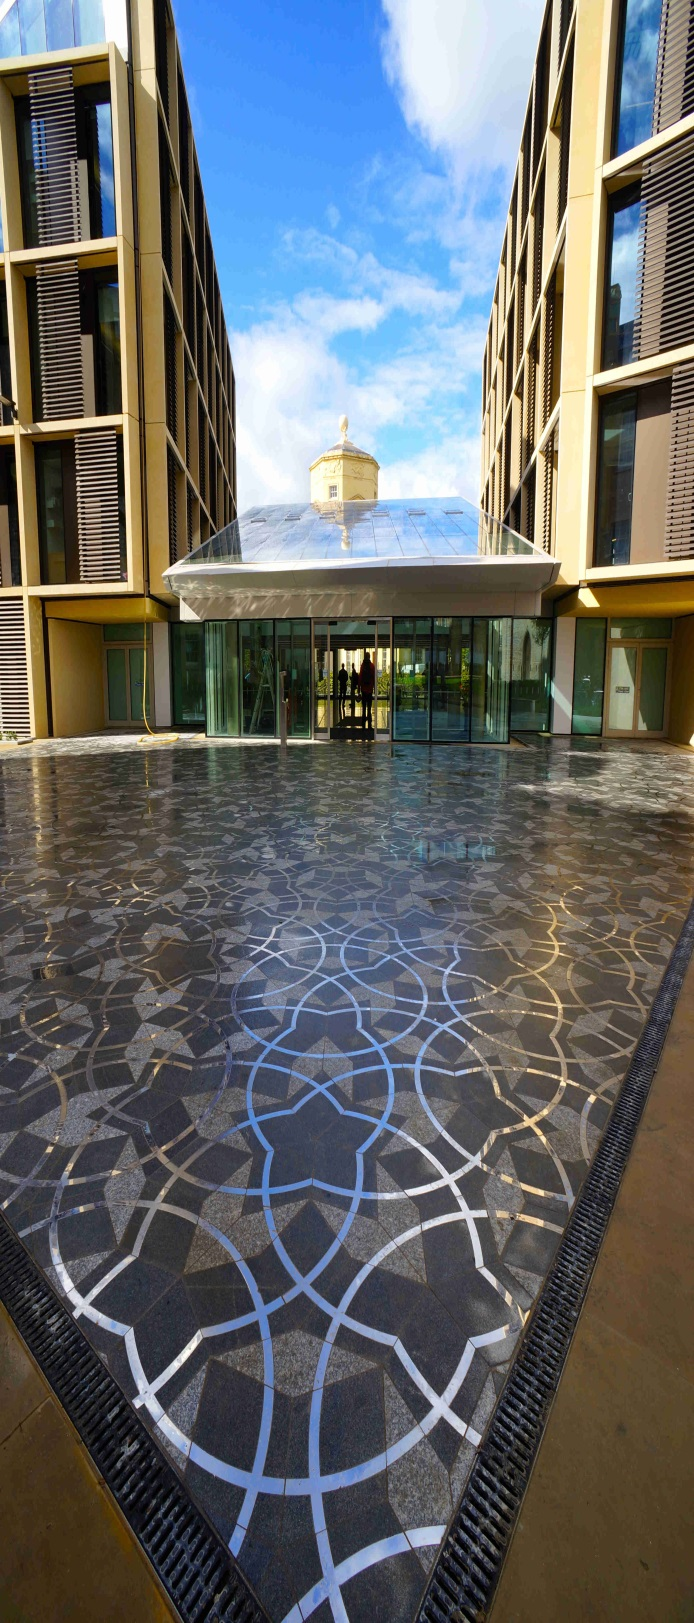
\includegraphics[width=\linewidth]{andrew_wiles_building}}
\clearpage
}
\iftoggle{TWOSIDED}{}{\reversemarginpar}
\cleardoublepage % Double page as page numbering starts at 1.
\setcounter{section}{0}
\pagenumbering{arabic}
